\documentclass[aspectratio=169]{beamer}
\usepackage{amsmath}
\usepackage{amssymb}
\usepackage{minted}
\usepackage{graphicx}
\title{EM algorithm}
\subtitle{Maximum Likelihood Estimation of the t-distribution}
\author{Lucas Støjko Andersen}
\setminted{fontsize=\fontsize{8pt}{8pt}}
\institute{University of Copenhagen}
\date{\today}

\begin{document}
\begin{frame}
    \titlepage
\end{frame}
\begin{frame} x
    \frametitle{The t-distribution}
    \framesubtitle{The density of the non-standard t-distribution}
    The density of the t-distribution is given by
    \begin{equation}
        \label{eq:marginal}
        g(x)=\frac{\Gamma\left(\frac{\nu + 1}{2}\right)}{\sqrt{\pi\nu\sigma^2}\Gamma\left(\frac{\nu}{2}\right)}\left(1+\frac{(x - \mu)^2}{\nu\sigma^2}\right)^{-\frac{\nu + 1}{2}}
    \end{equation}
    with parameters $\mu\in\mathbf{R}$, $\nu > 0$, $\sigma^2 > 0$. Here, $\Gamma$ is the gamma function.\\[12pt]
    For independent observations $X_{1},X_{2},\ldots,X_{n}$ with density as in (\ref{eq:marginal}) there exist no nice analytic solutions to the MLE --- even with $\nu$ known.
\end{frame}
\begin{frame}
    \frametitle{There is another way}
    \framesubtitle{A joint approach with latent variables}
    Consider $(X, W)$ with density
    \begin{equation}
        \label{eq:join}
        f(x,w)=\frac{1}{\sqrt{\pi\nu\sigma^2}2^{(\nu+1)/2}\Gamma(\nu/2)}w^{\frac{\nu - 1}{2}}e^{-\frac{w}{2}\left(1+\frac{(x -\mu)^2}{\nu\sigma^2}\right)}
    \end{equation}
    Notice that $W\mid X = x \sim \Gamma(\alpha, \beta)$ --- the gamma distribution --- with parameters
    \begin{equation}
        \alpha = \frac{\nu + 1}{2} \quad\quad 
        \beta = \frac{1}{2}\left(1+\frac{(x -\mu)^2}{\nu\sigma^2}\right).
    \end{equation}
    This can be used to show that $X$ indeed has the marginal density of the t-distribution with parameters $\mu,\sigma^2,\nu$.
\end{frame}
\begin{frame}
    \frametitle{The Full Maximum Likelihood Estimate}
    \framesubtitle{MLE with fixed $\nu$}
    Assume $\nu>0$ known. I.i.d. $(X_{1},W_{1}), (X_{2},W_{2}),\ldots,(X_{n},W_{n})$ have log-likelihood
    \begin{equation}
        \ell(\theta)\simeq -\frac{n}{2}\log\sigma^2 -\frac{1}{2\nu\sigma^2}\sum_{i=1}^{n}W_{i}(X_{i}-\mu)^{2}.
    \end{equation}
    The solution is that of the weighted least squares:
    \begin{equation}
        \hat\mu =\frac{\sum_{i=1}^{n}W_{i}X_{i}}{\sum_{i=1}^{n}W_{i}},\quad\quad \hat\sigma^2 = \frac{1}{n\nu}\sum_{i=1}^{n}W_{i}(X_{i}-\hat\mu)^{2}.
    \end{equation}
\end{frame}
\begin{frame}[fragile]
    \frametitle{The Full Maximum Likelihood Estimate}
    \framesubtitle{MLE with fixed $\nu$ --- implemented in R}
    We can sample $(X,W)$ by sampling $W$ from a $\chi^{2}_{\nu}$ distribution and then sampling $X$ from a $\mathcal{N}(\mu, \nu\sigma^2/W)$.

\begin{minted}{R}
simulate_X <- function(N, mu, sigma, nu) {
    W <- rchisq(N, nu)
    X <- rnorm(N, mu, sqrt(nu * sigma / W))
    
    list(x = X, w = W)
}
    
full_mle <- function(X, W, nu) {
    mu <- sum(X * W) / sum(W)
    sigma <- sum(W * (X - mu)^2) / (nu * (length(X)))
    list(mu = mu, sigma = sigma)
}

set.seed(3939392)
samples <- simulate_X(100000, 5, 1.5, 3)
full_mle(samples$x, samples$w, 3)
\end{minted}
We obtain the estimates $\hat\mu_{\text{full}} = 4.997852$ and $\hat\sigma^{2}_{\text{full}}=1.500886$.
\end{frame}
\begin{frame}
    \frametitle{EM algorithm}
    \framesubtitle{MLE of the marginal likelihood for fixed $\nu$}
    Only $X$ is observed and so the full MLE cannot be computed. Using the EM algorithm we iteratively maximize the quantity
    \begin{equation}
        Q(\theta\mid\theta')=E_{\theta'}(\log f_{\theta}(X, W)\mid X)
    \end{equation}
    where $\theta = (\mu,\sigma^2)$. Using the log-likelihood from earlier
    \begin{equation}
        Q(\theta\mid\theta')\simeq -\frac{n}{2}\log\sigma^{2}-\frac{1}{2\nu\sigma^{2}}\sum_{i=1}^{n}E_{\theta'}(W_{i}\mid X_{i})(X_{i}-\mu)^{2}.
    \end{equation}
    The maximizer is then
    \begin{equation*}
        \hat\mu_{\theta'} =\frac{\sum_{i=1}^{n}E_{\theta'}(W_{i}\mid X_{i})X_{i}}{\sum_{i=1}^{n}E_{\theta'}(W_{i}\mid X_{i})},\quad \hat\sigma^{2}_{\theta'}= \frac{1}{n\nu}\sum_{i=1}^{n}E_{\theta'}(W_{i}\mid X_{i})(X_{i}-\hat\mu)^{2}.
    \end{equation*}
\end{frame}
\begin{frame}
    \frametitle{EM algorithm}
    \framesubtitle{E-step and M-step}
    The E-step boils down to computing $E_{\theta'}(W_{i} \mid X_{i})$
    \begin{equation}
        E_{\theta'}(W_{i} \mid X_{i}) = \frac{\alpha}{\beta}=\frac{\nu' + 1}{2}\frac{1}{\frac{1}{2}\left(1 + \frac{(X_{i} - \mu')^{2}}{\nu'\sigma'^{2}}\right)}=\frac{\nu' + 1}{1 + \frac{(X_{i}- \mu')^{2}}{\nu'\sigma'^{2}}}
    \end{equation}
    and doing the M-step by computing
    \begin{equation*}
        \hat\mu_{\theta'} =\frac{\sum_{i=1}^{n}E_{\theta'}(W_{i}\mid X_{i})X_{i}}{\sum_{i=1}^{n}E_{\theta'}(W_{i}\mid X_{i})},\quad \hat\sigma^{2}_{\theta'}= \frac{1}{n\nu}\sum_{i=1}^{n}E_{\theta'}(W_{i}\mid X_{i})(X_{i}-\hat\mu)^{2}.
    \end{equation*}
\end{frame}
\begin{frame}[fragile]
    \frametitle{EM algorithm}
    \framesubtitle{Implementation of marginal MLE}

\begin{minted}{R}
E_step <- function(x, nu) {
    force(x)
    force(nu)
    function(par) {
        # mu = par[1]
        # sigma^2 = par[2]
        (nu + 1) / (1 + ((x - par[1])^2) / (nu * par[2]))
    }
}

M_step <- function(x, nu) {
  force(x)
  force(nu)
  function(EW) {
    mu <- sum(EW * x) / sum(EW)
    sigma <- mean(EW * (x - mu)^2) / nu
    c(mu, sigma)
  }
}
\end{minted}

\end{frame}
\begin{frame}[fragile]
    \frametitle{EM algorithm}
    \framesubtitle{Implementation of marginal MLE}

\begin{minted}{R}
EM <- function(par, x, nu, maxit = 500, min.eps = 1e-7) {
    E <- E_step(x, nu)
    M <- M_step(x, nu)
    for(i in 1:maxit) {
        EW <- E(par)
        new_par <- M(EW)
        if(sum((new_par - par)^2) < min.eps * (sum(par^2) + min.eps)) {
            par <- new_par
            break
        }
        par <- new_par
        if(i == maxit) warning("Maximum number of itertaions reached.")
    }
    names(par) <- c("mu", "sigma")
    list(par = c(par, nu = nu), iterations = i)
}
\end{minted}

\end{frame}

\begin{frame}
    \frametitle{EM algorithm}
    \framesubtitle{Comparison of marginal MLE and full MLE}
    For starting values $\theta' = (1, 2)$ we obtain the estimates
    \begin{equation}
        \hat\mu_{\text{EM}}=4.995958,\quad\quad \hat\sigma^{2}_{\text{EM}}=1.504293,\quad\quad \nu = 3.
    \end{equation}
    in 9 iterations of the EM algorithm. Recall the full MLE
    \begin{equation}
        \hat\mu_{\text{full}} = 4.997852, \quad\quad \hat\sigma^{2}_{\text{full}}=1.500886,\quad\quad \nu = 3.
    \end{equation}
\end{frame}

\begin{frame}
    \frametitle{Robustness of the initial parameters}
    \framesubtitle{Properties of the t-distribution}
    The t-distribution has first moment if $\nu > 1$ and second moment if $\nu > 2$. When the moments exist then
    \begin{equation}
        EX = \mu,\quad\quad VX = \sigma^{2}\frac{\nu}{\nu + 2}.
    \end{equation}
    The calculations in the E-step may be unstable
    \begin{equation*}
        \hat\mu_{\theta'} =\frac{\frac{1}{n}\sum_{i=1}^{n}E_{\theta'}(W_{i}\mid X_{i})X_{i}}{\frac{1}{n}\sum_{i=1}^{n}E_{\theta'}(W_{i}\mid X_{i})},\quad \hat\sigma^{2}_{\theta'}= \frac{1}{n\nu}\sum_{i=1}^{n}E_{\theta'}(W_{i}\mid X_{i})(X_{i}-\hat\mu)^{2}.
    \end{equation*}
\end{frame}

\begin{frame}[fragile]
    \frametitle{Robustness of the intial parameters}
    \framesubtitle{Gaussian resemblence of the t-distribution for large $\nu$}
    When $\nu\longrightarrow\infty$ the density of the t-distribution approaches the density of a normal distribution with mean $\mu$ and variance $\sigma^{2}$. It does so very quickly!
    \begin{figure}
        \centering
        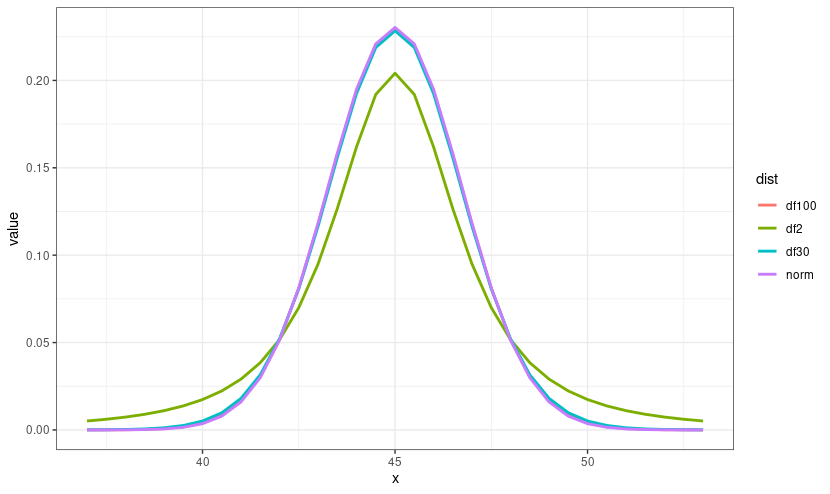
\includegraphics[scale=0.35]{pictures/densities.png}
        \caption{$\mu = 45$, $\sigma^{2}= 3$.}
    \end{figure}
\end{frame}
\end{document}
